%----------------------------------------------------------------------------
\chapter{Kiértékelés szintetikus adatokon}\label{chapter:kiertekelesszintetikus}
%----------------------------------------------------------------------------
% végére szekvenciadiagrammok, összehasonlítva az előző fejezet algoritmusával

Ez a fejezet bemutatja a korábbi fejezetekben ismertetett és implementált algoritmusok eredményét különböző általános adathalmazokon. Az ebből kapott eredményeket ismerteti és összehasonlítja egymással.

\section{Adatforrás}
A gépi tanulási algoritmusok bemenete általában egy adatsor. Egy megtisztított adatsort létrejötte egy hosszabb folyamat eredménye. Először adatfelvételt kell végezni, gyakran ezt digitalizálni is szükséges. Ezután a ki kell szűrni a mérési hibákat amennyire lehetséges. A cél egy olyan adatsor, amely nem tartalmaz hiányt és egyik változó szórása sem kiemelkedően magas.

Annak érdekében, hogy az új algoritmusok teszteléséhez, valamint az eredményeik reprodukálásához ne legyen szükség ezeknek a lépéseknek az elvégzésére, léteznek előfeldolgozott adatokat tartalmazó adatbázisok, melyek szabadon hozzáférhetők. Így a reprodukálás is egyszerűbb, mert ugyanazokon az adatokon lehet így futtatni az algoritmusokat.

Az egyik legismertebb és legtöbbet használt ilyen adatbázis az \emph{UCI Machine Learning Repository} \cite{dua2019university}. 1987-ben hozták létre egy ftp-n elérhető archívumként. Jelenleg 588 adatsort tartanak karban. Ismertsége megmutatkozik abban is, hogy a számítástechnikai publikációkban a 100 legtöbbet hivatkozott forrás között szerepel. Emellett a \emph{scikit-learn} python csomag, mely az adattudósok körében szintén gyakran használt könyvtár, több adatsort tartalmaz ebből a tárházból. Ezek a csomag telepítésével automatikusan letöltődnek, mert elég kis méretűek.

\section{Iris}
Az adattárház egyik első adatsora. A különböző nőszirom nemzetségbe tartozó fajokról tartalmaz információkat. Három faj szerepel benne: a mocsári írisz, a foltos nőszirom és a virginiai nőszirom. A fajok példányai a rekordok, mindegyik tartalmazza a példány csészelevelének és sziromlevelének a szélességét és magasságát. A cél megállapítani a növényfajt a kapott csésze- és sziromlevél méretekből.Minden fajhoz 50 adatpont tartozik, így a teljes adatsor 150 mintából áll. Mivel sok más tanulmánnyal is összevethetők így az adatok, az algoritmusok összehasonlításához ez a Diplomamunka is ezt az adatsort használja.

További előnye a kis változószám, amely miatt az eredmények könnyebben áttekinthetők.

\subsection{Referencia}
A Chen et al. \cite{chen2017learning} és a \ref{chapter:bayesdontesalapu}. fejezet által ismertetett módszer eredményei szerepelnek ebben a szakaszban. A tanulmányban leírt módokon futott, hogy az implementáció sikerességét empirikusan is meg lehessen tapasztalni. Az így kapott eredményeket össze lehet hasonlítani más tanulási módokkal, így a kiértékelésnél ez van először bemutatva.

A bemutatott két módszer egyike az ismert topológiai sorrendű struktúrán tanulás, a másik minden előzetes információ nélkül, a legjobb értékelésűt kiválasztva.

Az ismert topológiai sorrend a \emph{E, A, B, C, D} amennyiben az oszlopokat ábécé szerint nevezzük el. Tehát a faj az első, ennek leszármazottjait keressük. Ezzel a sorrenddel k2 struktúra tanulás fut, mely közben minden él hozzáadása után lefut a diszkretizáló algoritmus. A struktúra tanulás következő lépése már a frissített diszkretizációval rendelkező adatokkal számol.

Az előzetes információk nélküli tanulás esetén 50 véletlenszerű topológiai sorrenddel futott a k2 algoritmus. Minden él hozzáadása után ebben az esetben is diszkretizáció következett, a frissített diszkretizációs elv alapján számolt adatokon. Öt változó esetén az összes lehetséges topológiai sorrend $5! = 120$ lenne, így a futtatáskor csak 42\%-a van tesztelve. Ezért előfordulhat, hogy több futtatás esetén különböző az eredmény. A kapott 50 struktúrához a k2 algoritmus heurisztikája értékeinek összegét rendeli. Ez alapján a legmagasabb értékű lesz a kiválasztott sorrend és struktúra.

\begin{figure}[htp]
    \centering
    \includegraphics[width=12cm]{figures/result/ref_adott.png}
    \caption{Referencia módszer szerint, ismert topológiai sorrend mellett kialakított Bayes-háló}
    \label{fig:eredmeny-referencia-ismert}
\end{figure}

\begin{table}[htp]\centering
    \begin{tabular}{lcc}
    Változó               & Ismert     & Véletlenszerű \\ \hline
    Csészelevél hossz     & 5.45, 6.15 & 5.45, 6.15   \\
    Csészelevél szélesség & 2.95, 3.35 & 2.95, 3.35   \\
    Sziromlevél hossz     & 2.45, 4.75 & 2.45, 4.75   \\
    Sziromlevél szélesség & 0.80, 1.75 & 0.80, 1.75
    \end{tabular}
    \caption{Referencia módszer szerint, ismert és véletlenszerű topológiai sorrend mellett számolt referenciatartományok a folytonos változókra}
    \label{tab:eredmeny-referencia}
\end{table}

Az ismert topológiai sorrend melletti futás nagyon gyors volt. Az inicializáció és a végleges diszkretizáció között 1,937 másodperc telt el.

Az automatikus tanulás során az eltelt időre a korábbi ötvenszerese várható, hiszen azt az algoritmust futtatjuk ötvenszer. A 2 perc 11 másodperces futásidő ennél lényegesen hosszabb (2s * 20 = 100s = 1m 40s). Ennek oka, hogy az ezalatt tanult bayes-hálók bonyolultabbak, mint az ismert sorrendű egy szülős felépítése. Az algoritmus pedig a közös gyerek szüleit lassan diszkretizálja. A véletlenszerű struktúrák esetén pedig ilyenek könnyen előfordulhatnak.

\begin{figure}[htp]
    \centering
    \includegraphics[width=12cm]{figures/result/ref_random.png}
    \caption{Referencia módszer szerint, véletlenszerű topológiai sorrendből a legjobb mellett kialakított Bayes-háló}
    \label{fig:eredmeny-referencia-random}
\end{figure}

A véletlenszerű topológiai sorrendekből az algoritmus szerint a \emph{E, B, D, A, C} bizonyult a legjobbnak. Az ebből kialakított Bayes-háló struktúra a \ref{fig:eredmeny-referencia-random}. ábrán látható. Hasonló az ismert struktúrához, de a sziromlevél szélesség és a csészelevél hossza között összefüggést ismert fel. A kialakult diszkretizáció megegyezik az ismert sorrenddel számolt diszkretizációval, ezért tekinthetjük ezt a referencia diszkretizációnak.
% TODO: összefüggés ábrán

\subsection{Egyváltozós diszkretizáció}
Egy egyszerű módszer a folytonos adatsorból Bayes-háló tanulására az egyváltozós diszkretizáció. A \ref{chapter:jelenlegimodszerek}. fejezet ismertetett két egyszerű módszert ehhez a feladathoz. A nyomaték párosítás komplexitása miatt algoritmikusan nehezen megvalósítható. A tárgyterület-függő diszkretizáció pedig általánosan nem alkalmazható.

Az egyváltozós diszkretizáció után kapott diszkrét adatsor felhasználható a különböző struktúra tanuló algoritmusok bemeneteként. Ilyenkor elég egyetlen alkalommal futtatni a struktúra tanulást, hiszen a diszkretizációs algoritmus eredménye független a struktúrától. Az így kapott Bayes-hálót értékelhetjük.

\begin{table}[htp]\centering
    \begin{tabular}{lccc}
        Változó               & Referencia & Egyenlő hosszú & Egyenlő mintaszámú \\ \hline
        Csészelevél hossz     & 5.45, 6.15 & 5.50, 6.70     & 5.40, 6.30                              \\
        Csészelevél szélesség & 2.95, 3.35 & 2.80, 3.60     & 2.90, 3.20                              \\
        Sziromlevél hossz     & 2.45, 4.75 & 2.97, 4.93     & 3.00, 4.90                              \\
        Sziromlevél szélesség & 0.80, 1.75 & 0.90, 1.70     & 1.00, 1.60                              \\
    \end{tabular}
\caption{Egyváltozós diszkretizációk és a referencia eredménye: a diszkretizációs határok}
\label{tab:eredmeny-egyvaltozos}
\end{table}


Az egyenlő széles és az egyenlő mintaszámú diszkretizációk eredményét a \ref{tab:eredmeny-egyvaltozos}. táblázat ismerteti. Az intervallum határok között kisebb eltérések láthatók. Általában a referencia vágópontjai alacsonyabbak, mint az egyváltozós vágások. A futásidő rendkívül rövid, mivel egy diszkretizációs és egy struktúra tanuló lépés fut csak. Minden esetben 0.071 másodperc körüli idő alatt elkészült a Bayes-háló.

\begin{figure}[htp]
    \centering
    \includegraphics[height=12cm]{figures/result/eq_width-greedy.png} \hfill
    \includegraphics[height=12cm]{figures/result/eq_width-chowliu.png}
    \caption{Egyváltozós diszkretizáció Bayes-hálói. Balra az \emph{exact} és a \emph{greedy}, jobbra a \emph{Chow-Liu} algoritmus által tanult háló gráfja.}
    \label{fig:eredmeny-egyvaltozos}
\end{figure}

Négy különböző struktúra tanuló algoritmussal kiértékelve mindkét diszkretizációs elvet a \ref{fig:eredmeny-egyvaltozos}. ábrán látható Bayes hálók készültek az \emph{exact, greedy} és \emph{Chow-Liu} algoritmusokkal. A különbség kizárólag az élek irányában van, egymás transzponáltjai \cite{essam1970some}. A \emph{Chow-Liu} alapértelmezetten az első változóból indul, ezért a csészelevél hossz mindennek az őse. A \emph{k2} algoritmus (a \emph{E, A, B, C, D} topológiai sorrenddel) ugyanazt a hálót alkotta, mint a referencia esetben, ami a \ref{fig:eredmeny-referencia-ismert}. ábrán látható. Az algoritmusok eredménye a diszkretizációtól nem változott meg, a különbségek nem voltak ehhez elég erőteljesek.

\subsection{Eredmény}
Az algoritmusok értékelése az implementált értékelő kimenete alapján történt. A vizsgálat tízszeres kereszt-validációt alkalmazott. Ez azt jelenti, hogy a teljes adathalmaz $\frac{9}{10}$ része vesz részt egyszerre a Bayes-háló tanításában. A maradék $\frac{1}{10}$ rész csak a tanítás után van átadva a diszkretizálónak. Ilyenkor a folytonos változókat a tanult diszkretizációs elv alapján rendezi csoportokba. Ezután a diszkretizált értékek alapján a betanított Bayes-háló kiadja a célváltozó (eredetileg diszkrét változó) legvalószínűbb értékét. A kapott és a valós értékeket a meghatározott metrikák \cite{powers2020evaluation} szerint kiértékeli.

\begin{table}[htp]\centering
    \begin{tabular}{lccc}
        Metrika                         & Referencia & Egyenlő hosszú & Egyenlő mintaszámú \\ \hline
        Valódi pozitív                  & 139.00     & \textbf{147.00}         & 139.00             \\
        Hamis pozitív                   & 11.00      & \textbf{3.00}           & 11.00              \\
        Valódi pozitív arány            & 0.93       & \textbf{0.98}           & 0.93               \\
        Hamis felfedezési arány         & 0.07       & \textbf{0.02}           & 0.07               \\
        Pozitív prediktív érték         & 0.93       & \textbf{0.98}           & 0.93               \\
        Pontosság                       & 0.95       & \textbf{0.99}           & 0.95               \\
        Matthews korrelációs együttható & 0.89       & \textbf{0.97}           & 0.89               \\
        F-pontszám                      & 0.93       & \textbf{0.98}           & 0.93
    \end{tabular}
\caption{Kiértékelés eredménye egyváltozós diszkretizációk esetén. \textbf{Félkövérrel} az adott metrika szerinti legjobb eredmény szerepel.}
\label{tab:kiertekeles-egyvaltozos}
\end{table}

A kiértékelés eredménye a \ref{tab:kiertekeles-egyvaltozos}. táblázatban található. A struktúra tanuló algoritmus az elért eredményeken nem változtatott, csak a diszkretizáció módosított rajta. Látható, hogy az egyenlő mintaszám alapján készült diszkretizáció ugyanolyan pontszámot ért el, mint a referencia módszer. Az egyenlő hosszú intervallumokkal dolgozó pedig mindkettőnél sokkal pontosabb volt.

\begin{figure}[htp]\centering
    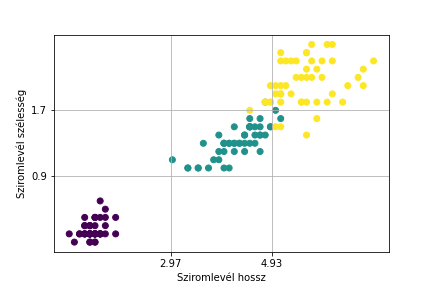
\includegraphics[width=12cm]{figures/IrisEloszlas.png}
    \caption{Iris adathalmaz sziromlevél hossz és sziromlevél szélesség változóinak együttes eloszlása az egyenlő hosszú diszkretizációs elv szerint. A különböző színek a különböző fajokat jelölik.}
    \label{fig:iris-eloszlas}
\end{figure}

Az egyenlő hosszú intervallumokkal dolgozó algoritmus jó eredményének az oka a \ref{fig:iris-eloszlas} ábrán látható. Ez az ábra az adatsor sziromlevél hossz, sziromlevél szélesség és faj változójának értékei alapján jelöli az adatpontokat. A két folytonos változó értéke határozza meg a pozíciót a grafikonon, míg a pont színe jelöli a fajt. A háttér vonalai az egyenlő hosszú diszkretizációs intervallum határokat jelölik.

Látható, hogy a két folytonos változó szerint a fajok elég nagy mértékben elkülönülnek. Az adatsor felépítése miatt, mivel minden fajból azonos mennyiségű példány szerepel, az egyenlő mintaszámú algoritmus ennyire elkülönülő csoportok esetén megtalálja a megfelelő határokat. A sárga és a zöldeskék pontok lineárisan nem szeparábilisek, ezért hibák mindegyik algoritmusnál előfordulnak. Az egyenlő hosszú algoritmusnak pedig "szerencséje" van ezzel az adatsorral, mert egy-egy folytonos változó egyenletes eloszlású és a fajok egy-egy harmadba esnek. Így sikerül jobb eredményt elérnie, mint a másik két eset.

Összefoglalva az látható, hogy egy egyszerű adathalmazon, melyben a minták jól elkülönülnek, a Bayes-döntés alapú diszkretizációs módszer nem tud jobb eredményt elérni, mint egy egyszerűbb algoritmus. Sőt, egyes esetekben jobb megoldást találhat egy egyváltozós diszkretizációs eljárás.

\section{Lakásár}
Ez az adatsor is az \emph{UCI Machine Learning Repository} adattárházból származik, 1993-ban töltötték fel oda. Boston agglomerációjának településeiről tartalmaz információkat. Sokkal összetettebb, mint az Iris adatsor, hiszen 14 változót tartalmaz. Emellett több adatpontja is van, szám szerint 506. Emiatt várhatóan az egyszerűbb algoritmusok nem lesznek képesek olyan jó eredményt elérni.

Két diszkrét változót tartalmaz, a \emph{Folyó} jelöli, hogy a Charles folyó környékén található-e, ez egy bináris változó. Valamint az \emph{Autópálya}, amely az elérhető autópályák számát jelöli. Ez 8 értéket vehet fel, ezért ez a vizsgálatban a célváltozó, amely alapján a kiértékelés történik. A folytonos változókból 12 van. A \emph{Bűnözés} jelöli a bűnözési rátát, a \emph{Zóna} a lakóövezetek aránya. A \emph{Föld} jelenti a településenkénti nem kiskereskedelmi üzleti földek arányát. A \emph{NO} a nitrogén-oxidok koncentrációja, \emph{Szoba} az átlagos szobaszám lakásonként, \emph{Tulajdonos} az 1940 előtt épült ingatlanokban a tulajdonos által használtak aránya. \emph{Távolság} a bostoni öt nagy foglalkoztató ügynökségtől vett távolságok súlyozott átlaga. \emph{Adó} a házra kiszabott vagyonadó mértéke, \emph{Tanár} a tanárok aránya a tanulókhoz, \emph{Etnikum} a kisebbségi etnikumúak aránya a településen. A \emph{Képzettség} az alacsonyan képzettek aránya végül a \emph{Medián} a tulajdonos által használt ingatlanok medián értéke.

A legnagyobb kardinalitású diszkrét változó ebben az adatsorban 8 értéket tartalmaz, így az algoritmusok célja is az adatok nagyjából nyolc intervallumra bontása. A változók sorrendjében az ABC betűi úgy vannak kiosztva, hogy a sorrend a folytonos változók felsorolásának rendje és a \emph{D} helyre a \emph{Folyó}, valamint az \emph{I} helyre a \emph{Autópálya} ékelődik be. Az ábrákon ezért a célváltozó az \emph{I}.

\subsection{Korábbi kísérletek}
A korábbi kísérleteket megismételve ezen az adatsoron látható, hogy itt sokkal jobban teljesített a referencia algoritmus (\ref{tab:kiertekeles-lakasar}. táblázat). Az ismert topológiai sorrend a \emph{D, E, G, B, H, C, I, M, N, J, A, F, K, L} lett, mert a leírt algoritmus szerint ez lett a legjobb. Azért térhet el a tanulmányban bemutatottól, mert csak 1000 véletlenszerű sorrend közül választja a legjobbnak ítéltet, 14 változó esetén pedig a lehetséges permutációk száma $14! \simeq 8.72 \cdot 10^{10}$.

Az ismert sorrenden az algoritmus 193.334 másodperc alatt, azaz 3 perc 13 másodperc alatt készítette el a betanított Bayes-hálót. Ez az időnövekedés egyrészt a mintapontok számának tudható be, hiszen az algoritmus $O(n^2)$ komplexitású a rekordok számára nézve. Másrészt a változók száma is nőtt, amely szintén $O(m^2)$ mértékben növeli a futásidőt. A k2 algoritmusban a szülők száma 3-ban maximalizálva volt, ezért nem magasabb rendű a komplexitás.

Az automatikus tanulás során tízszer futott véletlenszerű topológiai sorrenddel a referencia algoritmus. Ezek közül a legjobbnak a \emph{B, F, G, M, N, J, C, I, K, D, L, A, H, E} sorrend bizonyult.

\begin{table}[htp]\centering
    \begin{tabular}{lc}
            & Bűnözés                                                          \\ \hline
    Egyenlő hosszú     & 9.89,  19.78,    29.66,  39.55,  49.43,    59.32,  69.21,  79.09 \\
    Egyenlő mintaszámú & 0.04,  0.07,    0.11,  0.18,  0.36,    1.13,  4.54,  9.72       \\ \hline

    & Zóna                                                              \\ \hline
    Egyenlő hosszú     & 11.11,  22.22,    33.33,  44.44,  55.56,    66.67,  77.78,  88.89 \\
    Egyenlő mintaszámú & 0.00,  0.00,    0.00,  0.00,  0.00,    0.00,  20.00,  35.00
    \end{tabular}
\caption{A Bűnözés és Zóna változók egyváltozós diszkretizációjának eredménye.}
\label{tab:housing_egyszeru_intervallumok}
\end{table}

Az egyenlő hosszú és egyenlő mintaszámú diszkretizációs elv intervallumai a \emph{bűnözés} és a \emph{zóna} változókhoz a \ref{tab:housing_egyszeru_intervallumok}. táblázatban látható. Mivel az adatok eloszlása nem lineáris, így a két algoritmus által megállapított határok jelentősen különböznek. A zóna egyenlő mintaszámú diszkretizációjának több 0 határa is van. Ez alapján a változó értéke az esetek $\frac{6}{8}$ részében 0. Ez nem okoz gondot, mert ilyenkor mindegyik zérus érték az első osztályba tartozik, a másik 5 osztály pedig üres.

\begin{figure}[htp]
    \centering
    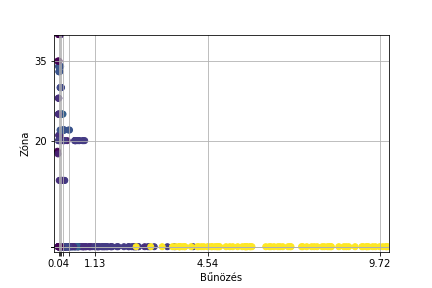
\includegraphics[width=12cm]{figures/housing_0_1_sample.png} \\
    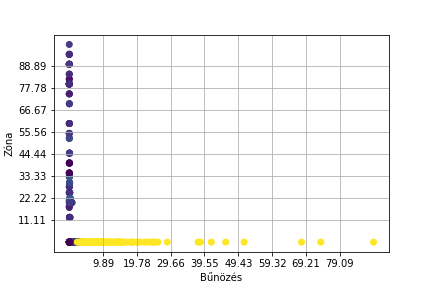
\includegraphics[width=12cm]{figures/housing_0_1_width.png}
    \caption{A Lakásár adathalmaz bűnözés és zóna változójának együttes eloszlása. Fent az egyenlő mintaszámú, lent az egyenlő hosszú diszkretizációs elv határai jelölve. A felső esetben esnek pontok a grafikonon kívülre is.}
    \label{fig:housing_eloszlas}
\end{figure}

A két változó együttes eloszlása a \ref{fig:housing_eloszlas}. ábrán látható. A színek az Autópálya változó értékét jelölik. Ebből leszűrhető, hogy magas bűnözés egy területre jellemző. Másrészt látványos, mennyire eltér a két diszkretizáció. Az egyenlő mintaszámúról több adatpont kilóg, mert azokat ábrázolva a diszkretizációs vonalak teljesen összecsúsznának. Ebből következtethetünk arra, hogy ott a kevés kiugró érték nagymértékben eltér a többitől.

Az eredmények között az egyenlő hosszú diszkretizáció a \emph{greedy} és a \emph{Chow-Liu} struktúra tanuló algoritmussal szerepel, az egyenlő mintaszámú pedig csak a \emph{Chow-Liu}-val. Az egyenlő mintaszámból tanulható esetek eredménye nagymértékben hasonló, az \emph{exact} algoritmus pedig mindkét esetben hasonló a \emph{greedy} algoritmushoz.

A futásidők itt jelentősen eltérnek. A \emph{Chow-Liu} algoritmus a kész struktúrával minden esetben 1 másodpercen belül visszatért, míg a másik kettőnek ehhez 3 percnél is több kellett. Ennek oka, hogy a \emph{Chow-Liu} a változók közötti függetlenséget statisztikai alapon gyorsan megállapítja, míg a többi algoritmusnak el kell végeznie a keresést, mely sok változónál és magas kardinalitásnál időigényes.

\subsection{K2 algoritmus kezdeti sorrend}
Ekkora változószám mellett és ilyen hosszú tanítási időkkel a Bayes-döntés alapú diszkretizáció lassú. Vagy nem talál meg egyetlen elfogadható topológiai sorrendet sem, mert túl keveset próbál ki, vagy a tanítási idő nő meg jelentősen. A \emph{Chow-Liu} gyors futásánál látható, hogy az információelméleti megközelítés ilyenkor is magas sebességet tud elérni. Ezért készültek olyan módszerek, melyek a topológiai sorrendet információelméleti alapon határozzák meg, és az így kapott sorrenddel futtatják a \emph{k2} algoritmust \cite{aghdam2019some}.

A feltételes entrópia alapú sorrend meghatározás implementálva van a \emph{bediscretizer} csomagban. Ezt használva a lakásár adatsoron a \emph{D, E, C, I, K, J, H, G, N, M, F, B, L, A} topológiai sorrend lesz az eredmény. Ezután futtatható a k2 algoritmus. A teljes futásidő 112.426 másodperc, tehát 1 perc 52 másodperc. Ez jobb, mint az ismert sorrenddel futó k2, aminek az oka, hogy kevés több szülős változó van a Bayes-hálóban. Ez nem az algoritmuson múlik, lehetett volna fordítva is, de az időkülönbséget magyarázza.

\subsection{Eredmény}

\begin{table}[htp]\centering
    \begin{tabular}{lcccccc}
        Metrika                         & \multicolumn{2}{c}{Referencia} & \multicolumn{2}{c}{Egyenlő hosszú} & \begin{tabular}[c]{@{}c@{}}Egyenlő\\ mintaszámú\end{tabular} & \begin{tabular}[c]{@{}c@{}}Kezdeti\\ sorrend\end{tabular} \\
                                        & Ismert     & Véletlen     & Greedy          & Chow-Liu         & Chow-Liu                                                     & K2                                                           \\ \hline
        Valódi pozitív                  & 450        & 457               & 314             & 296              & 398                                                          & \textbf{461}                                                          \\
        Hamis pozitív                   & 56         & 49                & 192             & 210              & 108                                                          & \textbf{45}                                                           \\
        Valódi pozitív arány            & 0.89       & 0.90              & 0.62            & 0.58             & 0.79                                                         & \textbf{0.91}                                                         \\
        Hamis felfedezési arány         & 0.11       & 0.10              & 0.38            & 0.42             & 0.21                                                         & \textbf{0.09}                                                         \\
        Pozitív prediktív érték         & 0.89       & 0.90              & 0.62            & 0.58             & 0.79                                                         & \textbf{0.91}                                                         \\
        Pontosság                       & 0.97       & \textbf{0.98}              & 0.91            & 0.91             & 0.95                                                         & \textbf{0.98}                                                         \\
        \begin{tabular}[c]{@{}l@{}}Matthews korrelációs\\ együttható\end{tabular} & 0.88       & 0.89              & 0.57            & 0.53             & 0.76                                                         & \textbf{0.90}                                                         \\
        F-pontszám                      & 0.89       & 0.90              & 0.62            & 0.58             & 0.79                                                         & \textbf{0.91}
        \end{tabular}
\caption{Kiértékelés eredménye a lakásár adatsoron. \textbf{Félkövérrel} az adott metrika szerinti legjobb eredmény szerepel.}
\label{tab:kiertekeles-lakasar}
\end{table}

Az algoritmusok az előző részben leírt módon, tízszeres kereszt-validációval lettek értékelve. Ez található a \ref{tab:kiertekeles-lakasar}. táblázatban. Látható, hogy az információelméleti alapon meghatározott kezdeti sorrend jól működött, szinte ugyanazt az eredményt érte el, mint az ismert sorrenden, valamint a többször futtatott véletlen sorrenden tanuló algoritmusok, ám a sebessége jobb azoknál. Az egyszerű algoritmussal számolt diszkretizációs elvek ennél az összetett adatsornál jobban lemaradtak a Bayes-döntés alapú diszkretizációs algoritmustól.

Az egyenlő mintaszámú diszkretizáció jobban teljesített az egyenlő hosszú intervallumoknál. Ennek oka, hogy az eredeti adatsor változóinak eloszlása jelentősen eltért az egyenletes eloszlástól. Emiatt az egyenlő hosszú intervallumok közül néhányba alig jutott adatpont, így kevésbé lehetett különbséget tenni és összefüggéseket felismerni.

%TODO: hálókról kép